\documentclass[tikz,border=3mm]{standalone}
\usepackage{fontspec}
\usetikzlibrary{arrows.meta,calc,decorations.pathreplacing,positioning}
\definecolor{ink}{HTML}{24323A}
\definecolor{slate}{HTML}{516672}
\definecolor{mist}{HTML}{EEF3F4}
\definecolor{sulfur}{HTML}{E7B928}
\definecolor{sulfurdark}{HTML}{9B6A00}
\definecolor{blue}{HTML}{277DA1}
\definecolor{cyan}{HTML}{63B7C6}
\definecolor{violet}{HTML}{7655A5}
\definecolor{red}{HTML}{C9503D}
\definecolor{green}{HTML}{3E8D72}
\tikzset{
  >={Latex[length=2.2mm,width=1.5mm]},
  txt/.style={font=\sffamily\scriptsize,text=ink},
  note/.style={font=\sffamily\tiny,text=slate},
  heading/.style={font=\sffamily\bfseries\small,text=ink},
  card/.style={draw=ink!25,fill=white,rounded corners=2mm,line width=.6pt},
  hero/.style={draw=blue!55,fill=blue!3,rounded corners=3mm,line width=1pt},
  arrow/.style={-{Latex[length=2.2mm]},line width=.9pt},
  satom/.style={circle,draw=sulfurdark,fill=sulfur,minimum size=3.2mm,
    inner sep=0pt,font=\sffamily\tiny,text=ink},
  charge/.style={circle,fill=red,text=white,minimum size=3mm,inner sep=0pt,
    font=\sffamily\bfseries\tiny}
}
\newcommand{\tagrole}[3]{
  \node[fill=#2,text=white,rounded corners=.8mm,minimum width=4.7mm,
    minimum height=4.7mm,font=\sffamily\bfseries\scriptsize] at (#1) {#3};
}
\begin{document}
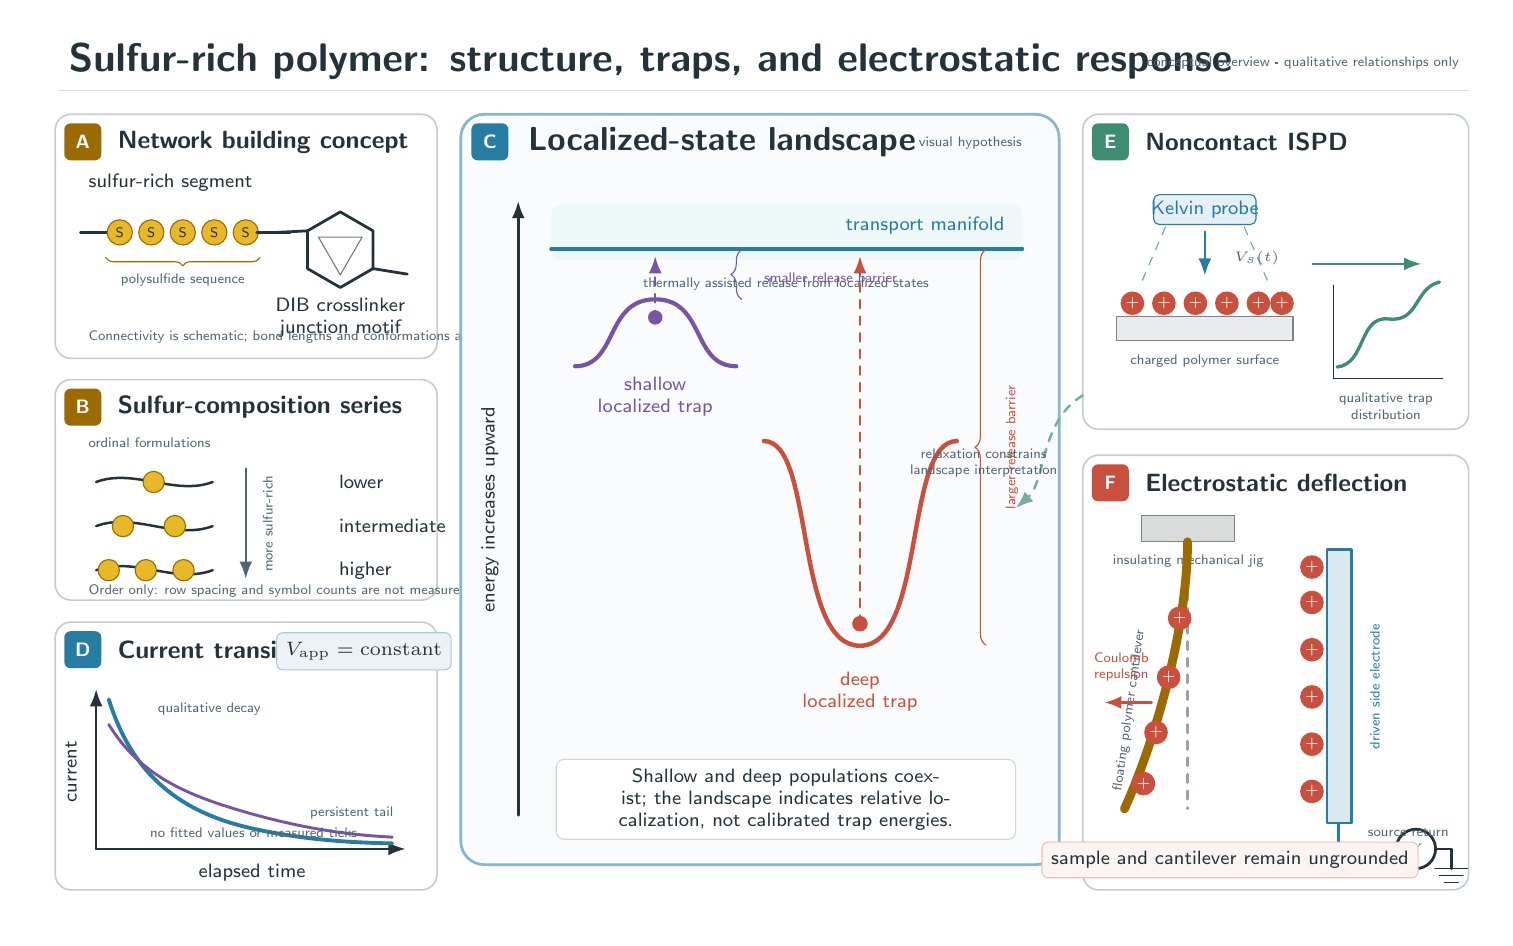
\begin{tikzpicture}[x=1cm,y=1cm,line cap=round,line join=round]

% Background and reading path
\fill[white] (-.15,-.15) rectangle (18.35,11.15);
\node[font=\sffamily\bfseries\Large,text=ink,anchor=west] at (.25,10.72)
  {Sulfur-rich polymer: structure, traps, and electrostatic response};
\node[note,anchor=east] at (18.15,10.70)
  {conceptual overview · qualitative relationships only};
\draw[ink!18] (.25,10.35)--(18.15,10.35);

% A — molecular concept, upper left
\draw[card] (.20,6.95) rectangle (5.05,10.05);
\tagrole{.55,9.70}{sulfurdark}{A}
\node[heading,anchor=west] at (.87,9.70) {Network building concept};
\node[txt,anchor=west] at (.50,9.18) {sulfur-rich segment};
\draw[ink,line width=1pt] (.52,8.55)--(.88,8.55);
\foreach \x in {1.02,1.42,1.82,2.22,2.62}{
  \node[satom] at (\x,8.55) {S};
}
\draw[ink,line width=1pt] (2.76,8.55)--(3.18,8.55);
\draw[decorate,decoration={brace,mirror,amplitude=3pt},sulfurdark]
  (.84,8.23)--(2.80,8.23);
\node[note] at (1.82,7.95) {polysulfide sequence};
\coordinate (ring) at (3.82,8.33);
\foreach \a in {30,90,...,330}
  \coordinate (r\a) at ($(ring)+(\a:.48)$);
\draw[ink,line width=1pt]
  (r30)--(r90)--(r150)--(r210)--(r270)--(r330)--cycle;
\draw[ink!65] ($(ring)+(30:.32)$)--($(ring)+(150:.32)$)
  --($(ring)+(270:.32)$)--cycle;
\draw[ink,line width=1pt] (r150)--(3.02,8.55);
\draw[ink,line width=1pt] (r330)--(4.67,8.02);
\node[txt,align=center] at (3.82,7.47) {DIB crosslinker\\junction motif};
\node[note,align=left,anchor=west] at (.50,7.22)
  {Connectivity is schematic; bond lengths and conformations are not modeled.};

% B — ordinal composition, lower left shoulder
\draw[card] (.20,3.88) rectangle (5.05,6.68);
\tagrole{.55,6.33}{sulfurdark}{B}
\node[heading,anchor=west] at (.87,6.33) {Sulfur-composition series};
\node[note,anchor=west] at (.50,5.88) {ordinal formulations};
\foreach \y/\lab in {5.38/lower,4.82/intermediate,4.26/higher}{
  \draw[ink,line width=.9pt] (.72,\y) .. controls (1.20,\y+.18)
    and (1.72,\y-.18) .. (2.20,\y);
  \node[txt,anchor=west] at (3.68,\y) {\lab};
}
\foreach \p in {(1.45,5.38),(1.06,4.82),(1.72,4.82),(.88,4.26),(1.35,4.26),(1.83,4.26)}
  \node[satom,minimum size=2.7mm] at \p {};
\draw[arrow,slate] (2.62,5.55)--(2.62,4.15);
\node[note,rotate=90] at (2.90,4.85) {more sulfur-rich};
\node[note,align=left,anchor=west] at (.50,3.99)
  {Order only: row spacing and symbol counts are not measurements.};

% D — transient current, lower left
\draw[card] (.20,.20) rectangle (5.05,3.60);
\tagrole{.55,3.25}{blue}{D}
\node[heading,anchor=west] at (.87,3.25) {Current transient};
\node[txt,fill=blue!9,draw=blue!40,rounded corners=.8mm] at (4.12,3.23)
  {$V_{\mathrm{app}}=\mathrm{constant}$};
\draw[arrow,ink] (.72,.72)--(.72,2.75);
\draw[arrow,ink] (.72,.72)--(4.65,.72);
\node[txt,rotate=90] at (.40,1.70) {current};
\node[txt] at (2.70,.42) {elapsed time};
\draw[blue,line width=1.4pt] (.88,2.62)
  .. controls (1.18,1.65) and (1.80,1.18) .. (2.70,.98)
  .. controls (3.42,.82) and (4.05,.80) .. (4.48,.79);
\draw[violet,line width=1.05pt] (.88,2.30)
  .. controls (1.30,1.62) and (1.92,1.38) .. (2.75,1.15)
  .. controls (3.52,.94) and (4.08,.89) .. (4.48,.87);
\node[note,anchor=west] at (1.38,2.50) {qualitative decay};
\node[note,anchor=east] at (4.62,1.18) {persistent tail};
\node[note,align=center] at (2.72,.93) {no fitted values or measured ticks};

% C — dominant trap-landscape hero
\draw[hero] (5.35,.52) rectangle (12.95,10.05);
\tagrole{5.72,9.70}{blue}{C}
\node[font=\sffamily\bfseries\large,text=ink,anchor=west] at (6.08,9.70)
  {Localized-state landscape};
\node[note,anchor=east] at (12.60,9.68) {visual hypothesis};
\draw[arrow,ink,line width=1.05pt] (6.08,1.15)--(6.08,8.95);
\node[txt,rotate=90] at (5.72,5.03) {energy increases upward};
\fill[cyan!10,rounded corners=1mm] (6.50,8.20) rectangle (12.48,8.90);
\draw[blue,line width=1.5pt] (6.50,8.34)--(12.48,8.34);
\node[txt,text=blue,anchor=east] at (12.38,8.63) {transport manifold};
\node[note,align=center] at (9.48,7.90)
  {thermally assisted release from localized states};
\draw[violet,line width=1.5pt]
  (6.80,6.85) .. controls (7.35,6.85) and (7.18,7.70) .. (7.82,7.70)
  .. controls (8.46,7.70) and (8.28,6.85) .. (8.85,6.85);
\fill[violet] (7.82,7.47) circle (2.6pt);
\draw[arrow,dashed,violet] (7.82,7.45)--(7.82,8.25);
\node[txt,text=violet,align=center] at (7.82,6.46) {shallow\\localized trap};
\draw[red,line width=1.6pt]
  (9.20,5.90) .. controls (9.85,5.90) and (9.58,3.30) .. (10.42,3.30)
  .. controls (11.26,3.30) and (10.98,5.90) .. (11.65,5.90);
\fill[red] (10.42,3.58) circle (2.8pt);
\draw[arrow,dashed,red] (10.42,3.58)--(10.42,8.25);
\node[txt,text=red,align=center] at (10.42,2.72) {deep\\localized trap};
\draw[decorate,decoration={brace,amplitude=4pt},violet]
  (8.92,7.70)--(8.92,8.33);
\node[note,text=violet,anchor=west] at (9.08,7.98) {smaller release barrier};
\draw[decorate,decoration={brace,amplitude=4pt},red]
  (12.02,3.31)--(12.02,8.33);
\node[note,text=red,rotate=90] at (12.35,5.82) {larger release barrier};
\node[txt,align=center,fill=white,draw=ink!20,rounded corners=1mm,
  text width=5.6cm] at (9.48,1.35)
  {Shallow and deep populations coexist; the landscape indicates relative
   localization, not calibrated trap energies.};

% E — ISPD links measurement to the hero
\draw[card] (13.25,6.05) rectangle (18.15,10.05);
\tagrole{13.60,9.70}{green}{E}
\node[heading,anchor=west] at (13.92,9.70) {Noncontact ISPD};
\fill[ink!10,draw=ink!60] (13.68,7.18) rectangle (15.92,7.48);
\node[note] at (14.80,6.91) {charged polymer surface};
\foreach \x in {13.88,14.28,14.68,15.08,15.48,15.78}
  \node[charge] at (\x,7.65) {$+$};
\draw[fill=blue!12,draw=blue,rounded corners=.7mm]
  (14.15,8.65) rectangle (15.45,9.03);
\node[txt,text=blue] at (14.80,8.84) {Kelvin probe};
\draw[dashed,blue!70] (14.30,8.62)--(13.98,7.88);
\draw[dashed,blue!70] (15.30,8.62)--(15.62,7.88);
\draw[arrow,blue] (14.80,8.56)--(14.80,8.00);
\node[note,anchor=west] at (15.05,8.23) {$V_s(t)$};
\draw[arrow,green] (16.17,8.15)--(17.55,8.15);
\draw[ink] (16.43,6.70)--(16.43,7.88);
\draw[ink] (16.43,6.70)--(17.82,6.70);
\draw[green,line width=1.2pt] (16.48,6.84)
  .. controls (16.85,6.88) and (16.75,7.50) .. (17.14,7.45)
  .. controls (17.52,7.41) and (17.46,7.84) .. (17.78,7.92);
\node[note,align=center] at (17.10,6.34) {qualitative trap\\distribution};
\draw[arrow,green!70,dashed] (13.25,6.48) .. controls (12.70,6.15)
  and (12.78,5.38) .. (12.40,5.05);
\node[note,align=center,anchor=east] at (13.05,5.62)
  {relaxation constrains\\landscape interpretation};

% F — correct vertical floating-cantilever geometry
\draw[card] (13.25,.20) rectangle (18.15,5.72);
\tagrole{13.60,5.37}{red}{F}
\node[heading,anchor=west] at (13.92,5.37) {Electrostatic deflection};
\fill[ink!18,draw=ink!60] (14.00,4.62) rectangle (15.18,4.95);
\node[note] at (14.59,4.38) {insulating mechanical jig};
\draw[ink!45,dashed,line width=1pt] (14.58,4.62)--(14.58,1.23);
\draw[sulfurdark,line width=3.2pt]
  (14.58,4.62) .. controls (14.58,3.58) and (14.20,2.16) .. (13.78,1.23);
\node[note,rotate=82,anchor=south] at (14.04,2.45) {floating polymer cantilever};
\draw[arrow,red,line width=1.2pt] (14.12,2.58)--(13.52,2.58);
\node[note,text=red,align=center] at (13.74,3.03) {Coulomb\\repulsion};
\fill[blue!18,draw=blue,line width=1pt] (16.35,1.05) rectangle (16.66,4.52);
\node[note,text=blue,rotate=90] at (16.96,2.78) {driven side electrode};
\foreach \y in {1.45,2.05,2.65,3.25,3.85,4.30}
  \node[charge] at (16.16,\y) {$+$};
\foreach \p in {(14.02,1.55),(14.18,2.20),(14.34,2.90),(14.48,3.65)}
  \node[charge] at \p {$+$};
\draw[blue,line width=1pt] (16.50,1.05)--(16.50,.72)--(17.23,.72);
\draw[ink,line width=1pt] (17.48,.72) circle (.25);
\node[note] at (17.48,.72) {$V$};
\draw[ink,line width=1pt] (17.73,.72)--(17.93,.72)--(17.93,.47);
\draw[ink] (17.72,.47)--(18.14,.47) (17.78,.38)--(18.08,.38)
  (17.84,.29)--(18.02,.29);
\node[note,anchor=east] at (18.02,.93) {source return};
\node[txt,fill=red!6,draw=red!35,rounded corners=.8mm,align=center]
  at (15.12,.58) {sample and cantilever remain ungrounded};

\end{tikzpicture}
\end{document}
